%%%%%%%%%%%%%%%%%%%%%%%%%%%%%%%%%%%%%%%%%%%%%%%%%%%%%%%%%%%%%%%%%%%%%%%%%%%%%%%%
%2345678901234567890123456789012345678901234567890123456789012345678901234567890
%        1         2         3         4         5         6         7         8

\documentclass[letterpaper, 10 pt, conference]{ieeeconf}  % Comment this line out if you need a4paper

%\documentclass[a4paper, 10pt, conference]{ieeeconf}      % Use this line for a4 paper

\IEEEoverridecommandlockouts                              % This command is only needed if 
                                                          % you want to use the \thanks command

\overrideIEEEmargins                                      % Needed to meet printer requirements.

%In case you encounter the following error:
%Error 1010 The PDF file may be corrupt (unable to open PDF file) OR
%Error 1000 An error occurred while parsing a contents stream. Unable to analyze the PDF file.
%This is a known problem with pdfLaTeX conversion filter. The file cannot be opened with acrobat reader
%Please use one of the alternatives below to circumvent this error by uncommenting one or the other
%\pdfobjcompresslevel=0
%\pdfminorversion=4

% See the \addtolength command later in the file to balance the column lengths
% on the last page of the document

% The following packages can be found on http:\\www.ctan.org
\usepackage{graphicx} % for pdf, bitmapped graphics files
%\usepackage{epsfig} % for postscript graphics files
%\usepackage{mathptmx} % assumes new font selection scheme installed
%\usepackage{times} % assumes new font selection scheme installed
\usepackage{amsmath}
\usepackage{amssymb}
\usepackage{booktabs}
\usepackage{bm}

\title{\LARGE \bf
Electronic Vehicle Battery Disassembly Using AgenticAI specifications
}


\begin{document}



\maketitle
\thispagestyle{empty}
\pagestyle{empty}


%%%%%%%%%%%%%%%%%%%%%%%%%%%%%%%%%%%%%%%%%%%%%%%%%%%%%%%%%%%%%%%%%%%%%%%%%%%%%%%%
\begin{abstract}

\end{abstract}


%%%%%%%%%%%%%%%%%%%%%%%%%%%%%%%%%%%%%%%%%%%%%%%%%%%%%%%%%%%%%%%%%%%%%%%%%%%%%%%%
\section{INTRODUCTION}
The continuous adoption of electronic vehicles (EV) poses a growing challenge in recycling their batteries \cite{beaudet2020key}, which contain a series of high-value materials that can often be recuperated to a large percentage in excess of 90\% \cite{ali2025sustainable}. With battery voltages now reaching 800V and a significant risk of a difficult-to-extinguish self-incineration due to thermal runway effects, manual disassembly is not only dull and dirty, but also dangerous. At the same time, economic incentives are dwindling: whereas current batteries are made of lithium, nickel, and cobalt (LNC), the new generation of mass-market batteries is based on lithium iron-phosphate (LFP), with raw materials costs of less than a quarter. This increases pressure on the industry to find solutions that reduce the cost of disassembly. One possible solution is to shred the entire battery. The resulting ``black mass'' is of lower quality, and therefore has a significantly lower price, than black mass that is obtained from shredding only the battery cells themselves \cite{choux2024shred}. Shredding the entire battery, including aluminum framing, copper busbars, and steel screws, also creates significant wear on the shredder gears that takes away from the unit economics of recycling. 
This has created considerable interest in robotic dismantling of EV battery cells.
An emerging technique is to cut the battery using lasers \cite{rettenmeier2024laser}. This is particularly important for so-called cell-to-pack architectures in which cells are not grouped into individual modules, but glued together into a large monolithic structure, as well as designs that extensively rely on welding of busbars instead of reversible connections. We consider cutting techniques to be complementary to robotic disassembly, in particular if reuse of components for remanufacturing is desired. 

Complete autonomy requires complex robotic systems that need to perform a large variety of tasks including screwing, cutting, prying, etc. In \cite{al2024automated}, a complete disassembly system for a hybrid battery is described and evaluated at the component disassembly level. Such systems usually require a large number of specialized tools, the ability to tool change, and specialized end-effectors to remove parts from the disassembly. For example, in \cite{huang2026robotic} a tool for automatically opening snap-fit connectors is presented and in \cite{tan2025robotic} a tool for removing screws after unscrewing is described. In \cite{qu2024robotic}, four robot arms, each with dedicated tools, are used for complete disassembly of a plug-in hybrid battery. Here, one robot can swap nuts on the nutrunner operated by the other robot. This work also directly compares dismantling times with that of a human operator, noting that robotic operations tend to be 20-30\% slower. 

In order to reduce the complexity of the robotic solution, others \cite{chen2014robot,wegener2015robot} propose a human-robot collaborative approach, using the Audi Q5 hybrid battery pack as an example, in which the robot is focused on repetitive screwing tasks, whereas the human is performing tasks that are more difficult to automate. 

Due to the large variety of tasks and battery packs, many of which require significant dexterity, we believe a human-robot collaborative approach to persist in industry and advocate a solution that can incrementally augment human assembly stations.  
\begin{figure}[t]
    \centering
    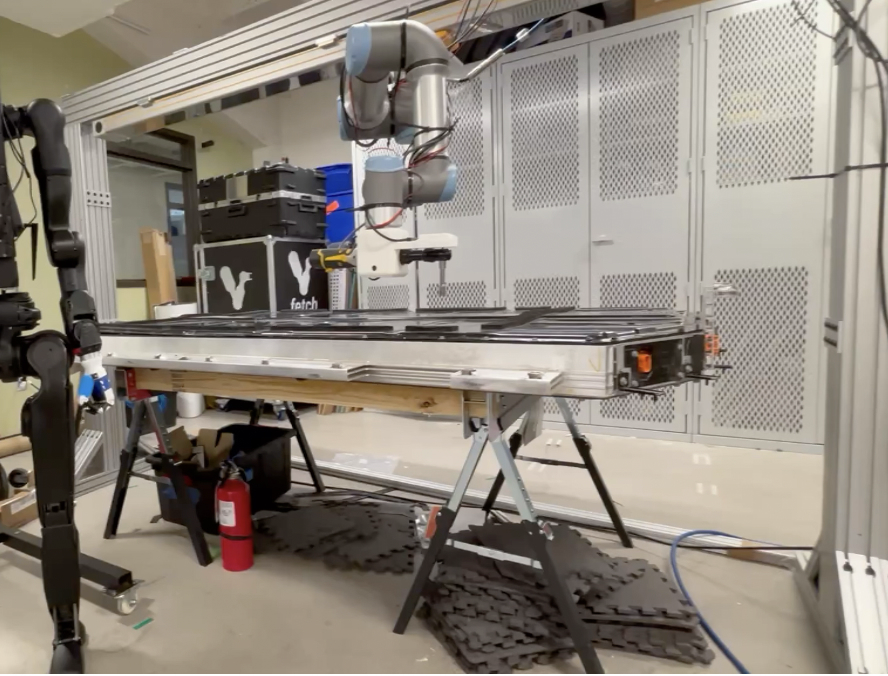
\includegraphics[width=0.9\columnwidth]{real.png}
    \caption{Hyundai Ioniq5 EV battery is being dismantled by a custom nut-runner mounted on a UR16e collaborative robot and a 2.1m Parker linear axis. \label{fig:overview}}
\end{figure}

\subsection{Related work}
We note that the majority of the related work is on the much smaller category of hybrid battery packs (usually small enough to fit in the area underneath the trunk) \cite{al2024automated,chen2014robot,wegener2015robot,qu2024robotic}, not on the emerging class of full-size EV battery packs that often span the entire chassis of the car, and operate at lower voltages (48V vs. 400-800V). These larger batteries exceed the workspace even of large industrial arms. The disassembly problem of \textit{packs} that consists of multiple \textit{modules}, should also not be confused with the disassembly of individual modules into \textit{cells} \cite{kay2022robotic}. 

In addition to performing specific tasks of the disassembly process \cite{huang2026robotic,tan2025robotic}, robotic disassembly taps into multiple areas of robotics such as task and motion planning. \cite{choux2021task} investigates a task planning framework for the complete disassembly of an Audi e-tron hybrid battery pack. Here, the planner is hard coding disassembly logic such as removing all visible screws before attempting the next step. In \cite{lee2022robot} a hierarchical planner is employed to disassemble a wooden toybox and an electronic hard-drive with emphasis on human-robot collaboration. In our work, we use Large Language Models (LLM) to interactively create a plan together with a human user. Here, LLMs can leverage common-sense knowledge about disassembly and also directly issue high-level commands to a robot's sensors and actuators \cite{raptis2025agentic}. In particular, LLMs can be used interactively to let a user refine a robotic manipulation plan \cite{lynch2023interactive}. In \cite{rachwal2025rai}, an Agentic AI framework has been presented that facilitates interactions between an LLM and sensors and actuators controlled by the Robot Operating System (ROS2). In addition to using the LLM to generate high-level plans, they also show using the LLM to detect anomalies during the execution of classical Finite State Machines (FSM), thereby potentially making robots more robust. 

Finally, \cite{hathaway2024technoeconomic} presents a techno-economic analysis of the battery disassembly process, computing cost savings larger than 40\% when using one Universal Robot arm to support dismantling of the Mitsubishi Outlander hybrid battery.  

\subsection{Contributions}
This paper presents a human-robot collaborative disassembly solution for a \textit{full-size} EV battery consisting of a robotic arm and overhead gantry system, as well as an agentic large language model approach to program and plan the disassembly system as well as collaborate with a human co-worker. s

\section{SYSTEM OVERVIEW}
 The dismantling system consist of a Universal Robot UR16e, a customized nut-runner (AlloyPower with custom Ethernet interface), and a Parker linear gantry.  Figure \ref{fig:real} shows the lab prototype with a Hyundai Ioniq5 full-size EV battery.  The end-effector is equipped with an Intel Realsense D435. Images are processed via Yolo World and motion planning is performed using MoveIt 2! \cite{coleman2014reducing}. The overall operation is orchestrated using an agentic AI framework SmolAgents \cite{smolagents}. Figure \ref{fig:overview} shows an overview of the system. 

\begin{figure}[thpb]
    \centering
    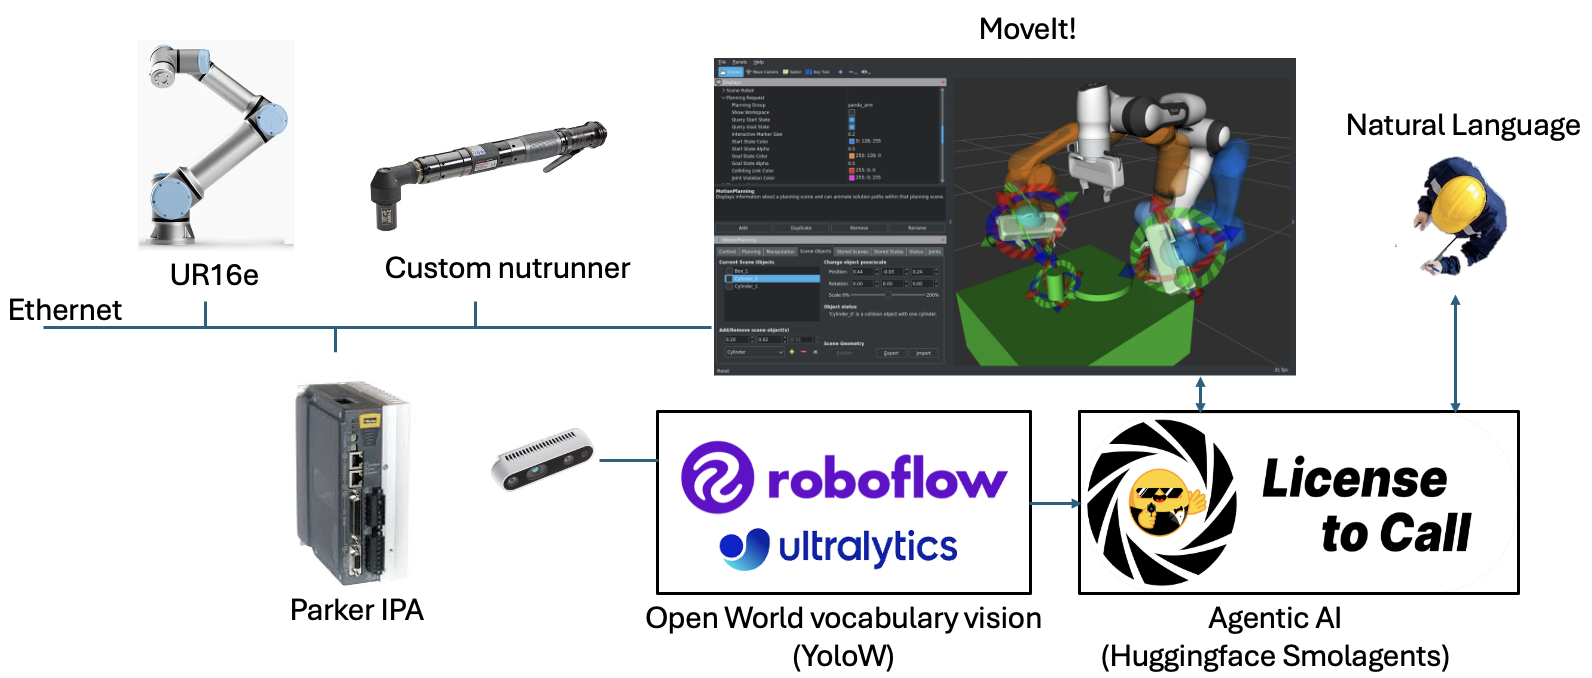
\includegraphics[width=\columnwidth]{overview.png}
    \caption{Integration of conventional automation systems, open-world vision systems, motion planning and Agentic AI. \label{fig:overview}}
\end{figure}

\subsection{Electric Vehicle Battery: Hyundai Ioniq5}
The Hyundai Ioniq5 is a full-size LNC EV battery that is 2.12m in length, 1.22m wide, weighs approximately 450kg, has a capacity of 77.4kWh, and operates at 800V. We have chosen this battery as it can be reversibly assembled and disassembled. Compared with hybrid or plug-in batteries, this kind of batteries require a much larger workspace, and additional safety precautions due to the high voltage, but has significantly different techno-economic benefits due to the increased amount of high-value materials. 

We have performed a complete manual disassembly of the battery to obtain an estimate of manual disassembly time using two untrained workers and a third person for time keeping who assisted in some of the tasks. We report and sum up the time required for all individual steps, not including breaks, and normalize them by ``man-hour'' and ``man-seconds''. Times were recorded after performing one complete disassembly and reassembly with the same team, somewhat reducing the effect of learning. Prior to disassembly, we have discharged the battery using an Webasto/Aeronvironment AV-900 Heavy Duty Dual Channel Cycling battery cycler to 0V. 

We identified 12 individual subtasks, which are listed in table \ref{tab:timing}. 
\begin{table*}[!htb]
\caption{Battery Disassembly Task Breakdown\label{tab:timing}}
\begin{center}
\begin{tabular}{|c|l|r|r|r|l|}
\hline
Task & Description & Time (s) & Workers & Man-seconds & Tools \\
\hline
1 & Remove 8 large screws on top cover & 120 & 2 & 240 & Large nutrunner \\
2 & Remove 70 screws and nuts holding top cover & 501 & 2 & 1002 & Nutrunner (high torque) \\
3 & Remove cover plate & 27 & 2 & 54 & None \\
4 & Remove two busbars to break battery voltage into two & 100 & 2 & 200 & Nutrunner (high torque) \\
5 & Remove two large cables connecting across battery & 173 & 2 & 346 & Nutrunner (high torque) \\
6 & Remove 6+1 large busbars & 190 & 2 & 380 & Nutrunner (high torque) \\
7 & Remove 3 busbars from battery controller & 136 & 2 & 272 & Nutrunner (high torque) \\
8 & Remove 8 wire harnesses & 420 & 2 & 840 & Small screwdriver, flathead \\
9 & Take out 24 small bus bars (battery module interconnects) & 456 & 2 & 912 & Nutrunner (high torque), small screwdriver \\
10 & Take out first layer of screws holding in battery modules (80 screws) & 960 & 2 & 1920 & Nutrunner (high torque) \\
11 & Take out second layer of M14 screws & 307 & 2 & 614 & Nutrunner (high torque) M14 \\
12 & Remove 32 battery modules & 343 & 3 & 1029 & Crowbar \\
\hline
\end{tabular}
\end{center}
\end{table*}

Table \ref{tab:materials} lists all of the components and their estimated recycling value. 

\begin{table*}[!htb]
\caption{Battery Component Weight and Material Values\label{tab:materials}}
\begin{center}
\begin{tabular}{|l|r|r|r|l|r|r|}
\hline
Part & Weight & Quantity & Total & Material & Price/kg & Total Value \\
\hline
Module & 11732g & 32 & 375.42kg & NCM Blackmass & \$3.50 & \$1,313.98 \\
Busbar S & 483g & 6 & 2.898kg & Copper & 7.06401766 & \$20.47 \\
M10 short/beefy & 14 &  & 0 & Steel & 0.15 & \$- \\
M10 long & 12 &  & 0 & Steel & 0.15 & \$- \\
M10 short & 6 &  & 0 & Steel & 0.15 & \$- \\
Small bus bars & 36 & 24 & 0.864 & Copper & 7.06401766 & \$6.10 \\
M14 & 13 &  & 0 & Steel & 0.15 & \$- \\
Top cover screws (large) & 109 & 8 & 0.872 & Steel & 0.15 & \$0.13 \\
Top cover screws (small) & 3 &  77 &   & Steel & 0.15 & \$- \\
Wire harness & 143g & 8 & 1.144 & Copper/insulation & 2.538631347 & \$2.90 \\
Top cover nuts &  & 78 & 0 & Steel &  & \$- \\
Other bus bars & 500g & 1 & 0.5 & Copper/insulation &  & \$- \\
Aluminium bottom & 60kg & 1 & 60kg & Aluminium & 1.103752759 & \$66.23 \\
Top cover & 3kg & 1 & 3kg & Steel & 0.15 & \$0.45 \\
\hline
\end{tabular}
\end{center}
\end{table*}

\subsection{Robotic System}
The robotic system has been dimensioned to service full-size EV batteries and consists of a T-slot arch spanning 2.5m in width, a Parker-Hannifin linear axis (2.1m) and an Universal Robots 16e 6-DoF robotic arm with a payload of 16 kg.  Both the  Intel RealSense D435 and the nut-runner are mounted using a custom, 3D-printed assembly shown in Figure \ref{fig:nutrunner}. Here, the camera is mounted slightly offset so that the nut-runner does not interfere with its field of view. The nut-runner is mounted so that its torque axis is perpendicular to the last axis of the robot, preventing reaction forces to be absorbed by the wrist. 

\begin{figure}
    \centering
    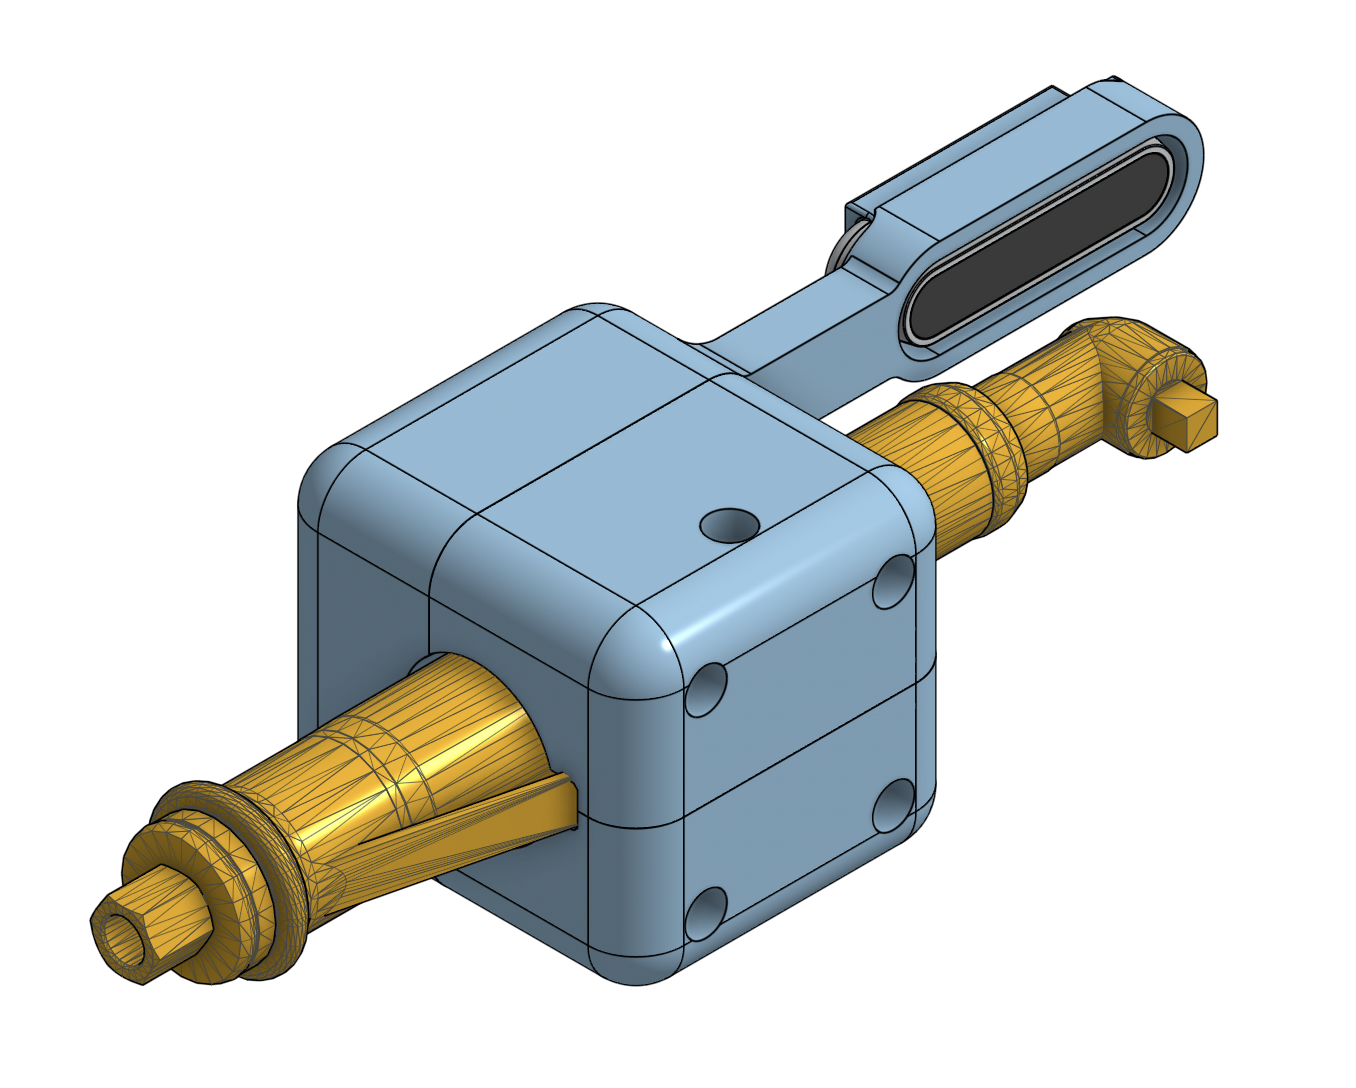
\includegraphics[width=0.7\columnwidth]{nutrunnerassembly.png}
    \caption{Custom end-effector for the UR16e that holds a nut-runner and a Intel Realsense D435 in place.    \label{fig:nutrunner}
}
\end{figure}

The UR16e provides a socket interface to send URScript commands. We have created custom scripts that allow us to move the robot toward a screw location in force control mode. Once the robot makes contact, the nut-runner is activated. As the nut-runner removes the screw, the robot automatically moves upward as it maintains a constant downward force. 

The nut-runner is equipped with a button that allows to regulate the nut-runner speed by modulating a pulse-width modulated (PWM) signal. We have replicated the built-in circuitry in order to control the nut-runner via an Ethernet connection. The schematic is shown in Figure XX. 

The gantry system can be controlled by sending assembler-like commands via another socket connection. It is equipped with an absolute encoder, which allows to move it with millimeter accuracy. 

The overall system is controlled by MoveIt! \cite{coleman2014reducing}, which implements path planning and collision avoidance. To this end, we are scanning the entire battery using the Intel Realsense to create a point-cloud collision object. 

\section{AUTONOMOUS DISASSEMBLY}
We envision the following industrial workflows: A preliminary setup sequence that will need to be done only once for every battery type

\begin{enumerate}
\item Scanning the battery, 
\item Manually labeling all relevant parts,
\item Training a vision model,
\item Map all relevant parts using vision and store their location in a database,
\item Manually annotate missing parts,
\item Create disassembly plans by providing text input,
\end{enumerate}

and the actual disassembly sequence,

\begin{enumerate}
\item Scan the entire battery and create a collision object,
\item Use vision to register the battery pose,
\item Execute the disassembly plan by issuing commands to both the robot and the worker,
\item Wait for worker input to continue the disassembly plan.
\end{enumerate}

We describe the details of the individual steps in the sections below.

\subsection{Planning}\label{sec:planning}
We formulate the sequencing of disassembly tasks as a Traveling Salesman Problem (TSP) defined over task poses in $SE(3)$. Let 
$$
T_s = \{t_{s,1}, \dots, t_{s,n}\}
$$
denote the set of disassembly tasks that are associated with step $s \in \mathcal{S}$, and $t_{s,0}$ represents the robot home configuration. Each task pose is defined as
$$
t_{s,i} = (p_{s,i}, q_{s,i}) \in SE(3),
$$
where $p_{s,i} \in \mathbb{R}^3$ is the Cartesian position and $q_{s,i} \in \mathbb{H}$ is a unit quaternion representing orientation. The augmented node set is
$$
V_s = \{t_{s,0}\} \cup T.
$$
Rather than defining edge costs through a geometric distance in task space, which does not reflect planning constraints, we construct a weight matrix
$$
W_{s,ij} \in \mathbb{R}_{\ge 0}, \quad i,j \in V_s,
$$
where each entry represents the minimum joint-space motion cost between task poses $t_{s,i}$ and $t_{s,j}$. Specifically, let
$$
\mathcal{Q}_{s,ij} = \{ q_{s,ij}^{(1)}, \dots, q_{s,ij}^{(N)} \}
$$
denote a set of $N$ inverse kinematic solutions for reaching pose $t_{s,j}$ from pose $t_{s,i}$, obtained via RRT* in joint space. The edge weight is then defined as
$$
W_{s,ij} = \min_{k \in \{1,\dots,N\}} \; c\!\left(q_{s,ij}^{(k)}\right)
$$
where $c(\cdot)$ denotes the joint-space path cost (e.g., path length, time, or energy). Note that $W_{s,ij}$ can be computed offline as the set of tasks $T$ is the same for each battery of the same type. 

The TSP decision variables are
$$
x_{s,ij} \in \{0,1\}, \quad i,j \in V,
$$
with $x_{s,ij}=1$ if the robot moves directly from $t_{s,i}$ to $t_{s,j}$. The optimization problem is
$$
\min_{x_{s,ij}} \sum_{i \in V} \sum_{j \in V} W_{s,ij} \, x_{s,ij},
$$
subject to the degree constraints
$$
\sum_{j \in V_s} x_{s,ij} = 1,  \quad
\sum_{i \in V_s} x_{s,ij} = 1 \quad \forall i,j \in V,
$$
and standard subtour elimination constraints ensuring a single Hamiltonian circuit. This formulation decouples global task sequencing from local motion planning while incorporating realistic joint-space motion costs into the routing objective and can be solved using Google's OR tools \cite{cuvelier2023or}.

\subsubsection{Analytical Inverse Kinematics}
Standard MoveIt-compatible solvers such as KDL, TracIK, and PICK-IK treat the linear actuator as an additional joint in an over-actuated chain and return a single, seed-dependent solution per call. For our 7-DoF system this is insufficient: different gantry positions give rise to qualitatively different arm configurations, and a single iterative call cannot enumerate them. We therefore implement a custom closed-form solver that exploits the UR16e's spherical wrist to decouple the position and orientation subproblems, and explicitly sweeps candidate gantry positions to cover the full workspace.

The 7-DoF system (6-DoF UR16e plus 1-DoF linear gantry) admits a closed-form IK solution for the arm at each fixed gantry position. We exploit the UR16e's spherical wrist to decompose the problem into five sequential subproblems: two shoulder-pan solutions from the horizontal wrist-center position, two wrist-2 solutions from the $z$-axis rotation constraint, and two elbow configurations from the resulting planar 2R inverse kinematics, yielding up to eight analytical solutions per gantry position. To cover the extended workspace, the analytical solver is evaluated at up to 21 candidate gantry positions, offset from the current position in 0.1\,m increments across $\pm 1.0$\,m and clamped to the actuator travel limits. Solutions are filtered by joint limits, a minimum end-effector clearance of 0.65\,m from the gantry plate, and a triangle-area validity check on the wrist--forearm--gantry triangle to reject near-singular configurations. This procedure typically generates 50--100 valid IK candidates per target pose.

\subsubsection{Multi-Objective IK Seed Selection}
To select the best IK solution for the motion planner, we define a composite cost function over three normalized objectives. Let $\bm{q}_c$ denote the current joint configuration and $\bm{q}_k$ a candidate IK solution. The raw cost components are:
\begin{itemize}
\item \textit{Joint distance}: weighted Euclidean distance $d_J(\bm{q}_c, \bm{q}_k) = \sqrt{\sum_{i=1}^{7} w_i (q_{c,i} - q_{k,i})^2}$, where $w_1 = 0.1$ (gantry) and $w_{2\text{--}7} = 1.0$ (arm joints), penalizing large joint-space motions while permitting gantry travel.
\item \textit{Proximity penalty}: $p_P = 1/d_{\text{ee}}$, where $d_{\text{ee}}$ is the Euclidean distance between the wrist and gantry plate links, discouraging configurations where the arm operates close to the gantry.
\item \textit{Area penalty}: $p_A = 1/A_\triangle$, where $A_\triangle$ is the area of the triangle formed by the gantry plate, wrist, and forearm links. Small triangle areas correspond to near-singular, collapsed arm configurations and serve as a geometric proxy for manipulability.
\end{itemize}
Each component is independently normalized to $[0,1]$ across all valid candidates and combined as
$$
C(\bm{q}_k) = \alpha \,\hat{d}_J + \beta \,\hat{p}_P + \gamma \,\hat{p}_A,
$$
where $\alpha$, $\beta$, $\gamma \geq 0$ are user-configurable weights exposed as runtime parameters. The candidate with the lowest $C(\bm{q}_k)$ is used as the IK seed for the sampling-based motion planner.

We additionally compute the Yoshikawa manipulability index $\mu = \sqrt{\det(\bm{J}\bm{J}^T)}$, where $\bm{J} \in \mathbb{R}^{6 \times 7}$ is the geometric Jacobian, for each planned configuration. While $\mu$ is not directly incorporated into the cost function, it is recorded as a diagnostic metric to quantify the dexterity of the selected configuration. We observe empirically that the area penalty $p_A$ correlates with manipulability, as collapsed arm triangles coincide with near-singular Jacobians.

\subsubsection{Corridor Constraint}
To produce predictable, human-safe motions in the collaborative workspace, we constrain the end-effector path to lie within a rectangular corridor between the start and goal poses. The corridor is defined as a 3D box whose long axis is aligned with the start-to-goal direction vector, with length equal to the segment distance plus a padding of $2 \times 0.25$\,m, and a square cross-section of $2 \times 0.5$\,m per side. The box is centered at the midpoint between start and goal and enforced as a MoveIt position constraint on the end-effector link.

\subsection{Vision}\label{sec:vision}
\subsection{Agentic AI}\label{sec:agenticAI}

\section{RESULTS}
WE NEED SOME RESULTS ON THE PLANNER. FOR EXAMPLE, WE COULD PLOT THE OVERALL PATH LENGTH AS A FUNCTION OF N=1,2,3...k IK SOLUTIONS.

We have measured accuracy for true-positive detection and intersection-over-unions (IoU) for X objects in the battery. We obtain XX\% accuracy and XX\% IoU on average. We can detect screws with accuracy XX, busbars with YY...

We have also timed a disassembly sequence for the top cover, by performing disassembly N=5 times. 


\subsection{Planning}
We evaluate the motion planner in two studies using 1{,}000 randomly sampled goal poses within the battery workspace, with a planning timeout of 20\,s. All metrics are averaged over successful plans only.

\subsubsection{RRT vs.\ Corridor-Constrained Planning}
We first compare unconstrained RRT planning against corridor-constrained planning (Section~\ref{sec:planning}) using 1{,}000 goals at a fixed height of $z = 1.31$\,m. Table~\ref{tab:rrt-corridor} summarizes the results. RRT achieves a higher success rate (99.1\% vs.\ 93.4\%) with dramatically lower planning times (0.09\,s vs.\ 29.87\,s on average). However, the corridor constraint produces more direct paths, with a path efficiency of 0.910 compared to 0.823 for unconstrained RRT.

\begin{table}[!t]
\caption{RRT vs.\ corridor planning comparison (avg.\ over successful plans).}
\label{tab:rrt-corridor}
\centering
\begin{tabular}{l ccccc}
\toprule
Strategy & SR (\%)$\uparrow$ & Plan (s)$\downarrow$ & Exec (s)$\downarrow$ & Path (m)$\downarrow$ & Eff.$\uparrow$ \\
\midrule
Pure RRT & \textbf{99.1} & \textbf{0.09} & \textbf{3.64} & 1.47 & 0.823 \\
Corridor & 93.4 & 29.87 & 6.97 & \textbf{1.26} & \textbf{0.910} \\
\bottomrule
\end{tabular}
\end{table}


Figure~\ref{fig:plantime-hist} shows the plan time distributions on a logarithmic scale. RRT plan times cluster tightly around 0.10\,s, while corridor-constrained planning exhibits a broad distribution with a median of 13.75\,s, with many plans approaching or exceeding the 20\,s timeout.

\begin{figure}[!t]
\centering
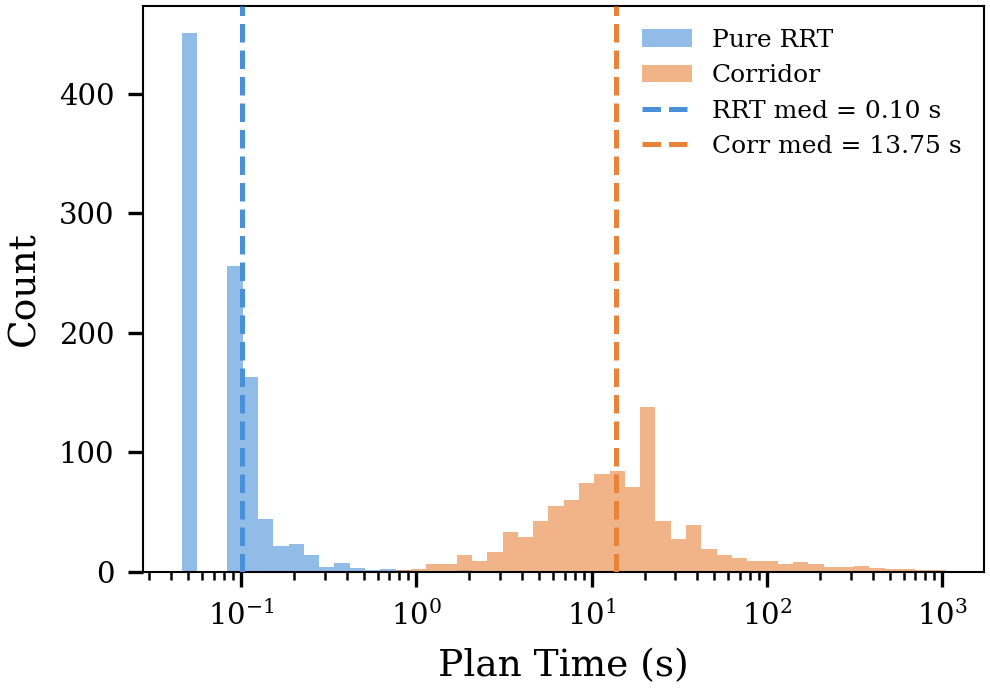
\includegraphics[width=\columnwidth]{fig_rrt_corridor_hist.png}
\caption{Plan time distributions for unconstrained RRT vs.\ corridor-constrained planning. Dashed line indicates the 20\,s timeout.}
\label{fig:plantime-hist}
\end{figure}

Figure~\ref{fig:plantime-scatter} shows a per-goal comparison of plan times. Nearly all points lie above the diagonal, confirming that the corridor constraint increases planning time for every goal. Blue points indicate goals where only RRT succeeded, predominantly at high corridor plan times where the constrained planner timed out.

\begin{figure}[!t]
\centering
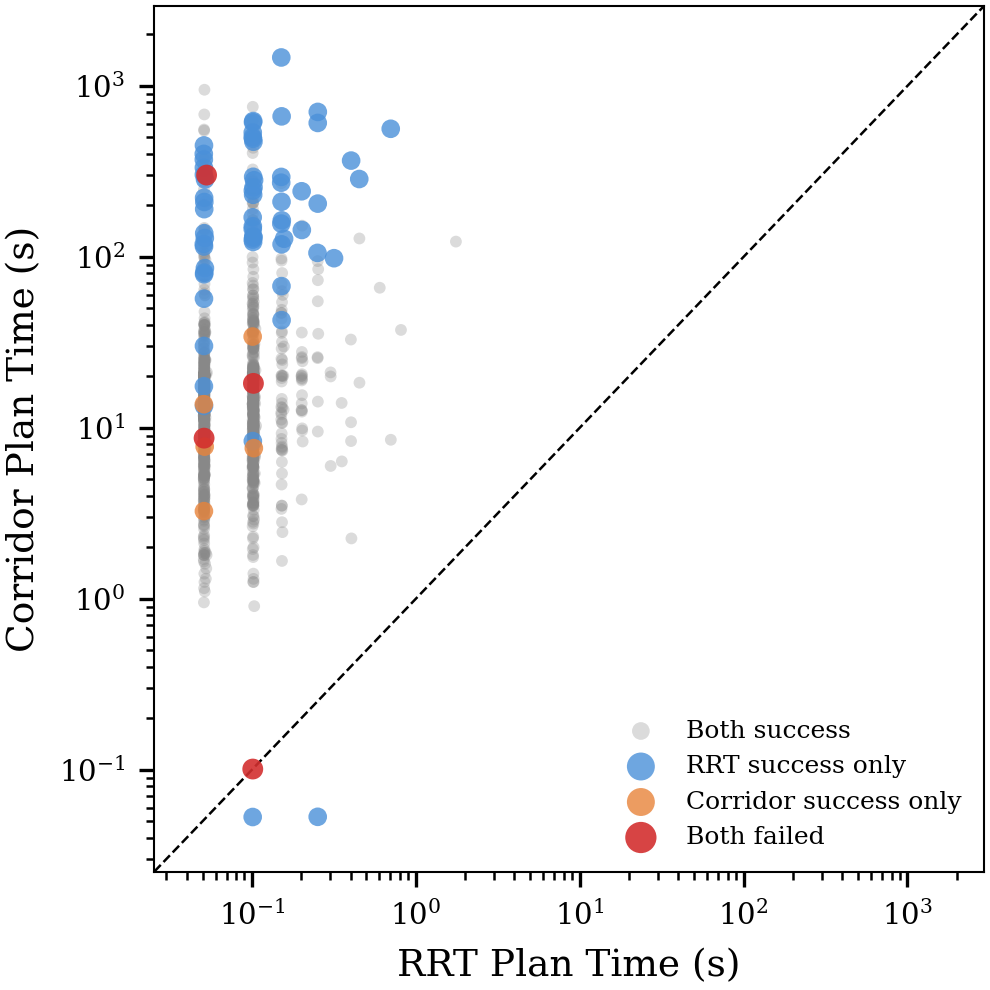
\includegraphics[width=\columnwidth]{fig_plantime_scatter.png}
\caption{Per-goal plan time comparison. Each point represents one of 1{,}000 goals. Points above the diagonal indicate corridor planning was slower.}
\label{fig:plantime-scatter}
\end{figure}

Figure~\ref{fig:spatial-failures} shows the spatial distribution of failures. RRT failures (9 total) are scattered, while corridor failures (66 total) cluster at the positive-$x$ workspace boundary, where the corridor box extends beyond the reachable workspace.

\begin{figure*}[!t]
\centering
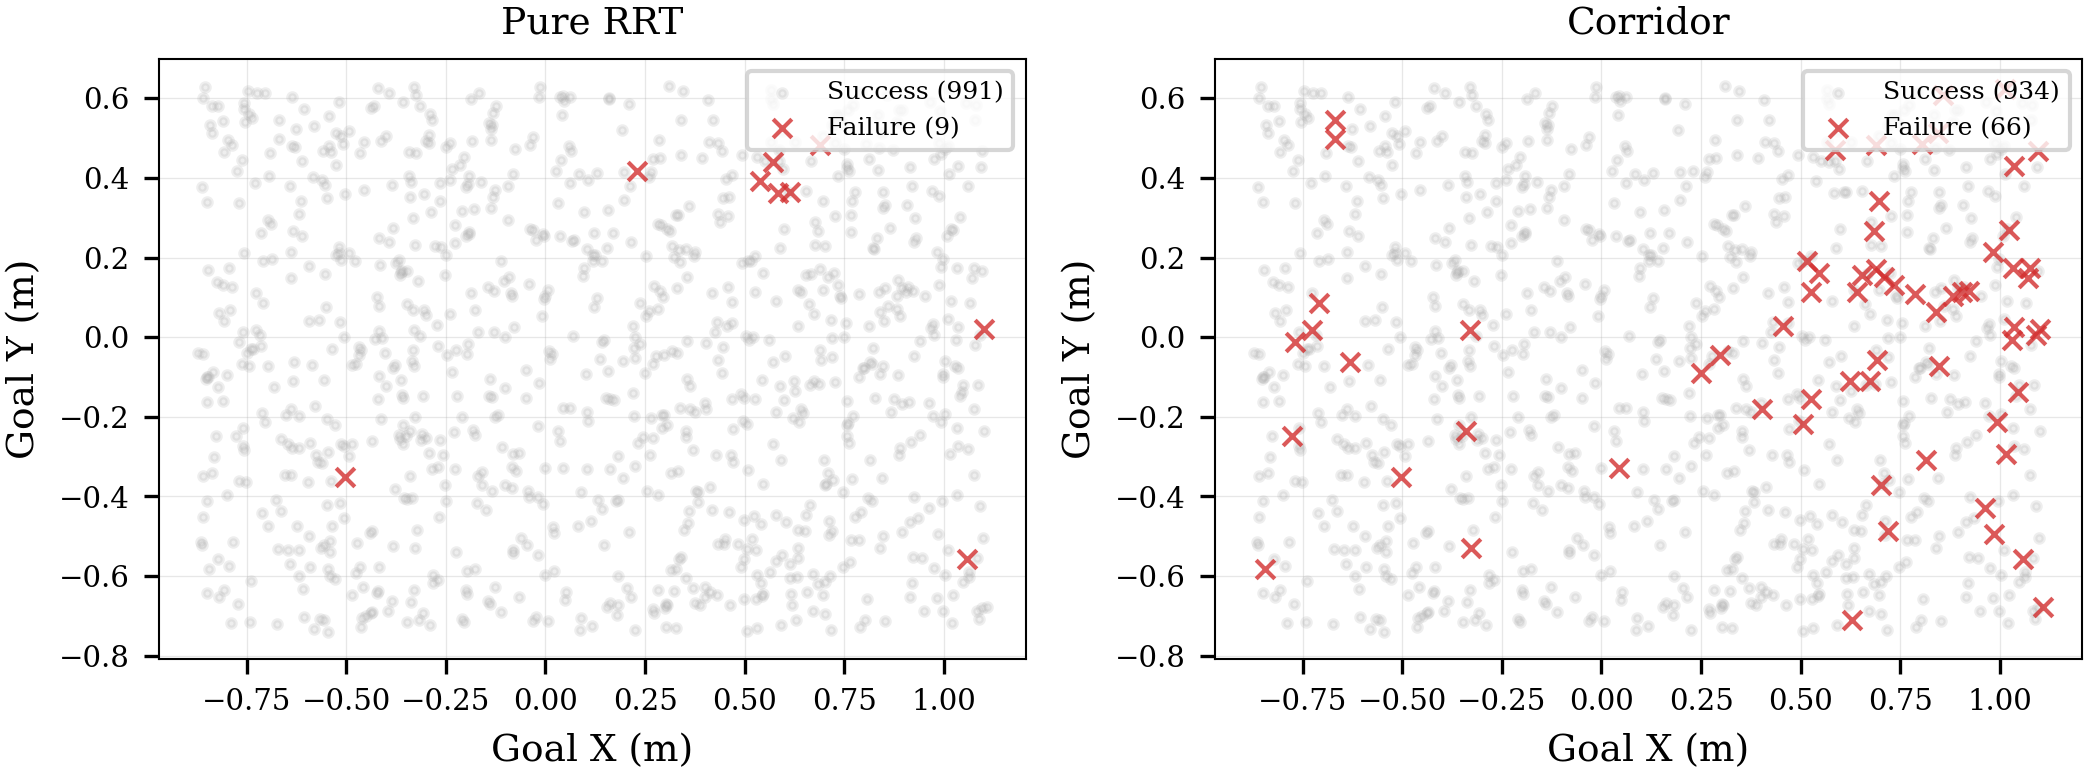
\includegraphics[width=\textwidth]{fig_spatial_failures.png}
\caption{Spatial distribution of planning failures. Left: unconstrained RRT (9 failures). Right: corridor-constrained planning (66 failures), with failures concentrated at the workspace boundary.}
\label{fig:spatial-failures}
\end{figure*}

\subsubsection{Cost Function Ablation Study}
We evaluate the effect of the three IK seed selection cost components (joint distance, proximity penalty, area penalty) using eight weight configurations in an ablation study. Goals are sampled with varying heights ($z \in [1.0, 1.47]$\,m) and planned from a fixed home position. Table~\ref{tab:cost-ablation} summarizes the results.

\begin{table}[!t]
\caption{Cost function ablation results (avg.\ over successful plans).
\textbf{Bold} = best, \underline{underline} = second best.}
\label{tab:cost-ablation}
\centering
\resizebox{\columnwidth}{!}{%
\begin{tabular}{l ccccc}
\toprule
Config. & SR (\%)$\uparrow$ & Plan (s)$\downarrow$ & Exec (s)$\downarrow$ & Path (m)$\downarrow$ & Manip.$\uparrow$ \\
\midrule
Base & \textbf{99.6} & 0.96 & 6.24 & 2.40 & 0.481 \\
\midrule
Area & 99.0 & 0.53 & 6.28 & 2.52 & 0.421 \\
Joint & 98.3 & 0.56 & 4.53 & \underline{1.64} & 0.489 \\
Prox & 99.3 & 0.38 & 4.24 & 1.87 & \textbf{0.700} \\
\midrule
~Area & \underline{99.4} & 0.48 & 4.33 & 1.78 & \underline{0.699} \\
~Joint & 99.1 & \underline{0.27} & 4.26 & 2.01 & 0.642 \\
~Prox & 97.9 & 0.27 & \textbf{3.98} & \textbf{1.52} & 0.424 \\
Equal & 99.3 & \textbf{0.22} & \underline{4.10} & 1.70 & 0.628 \\
\bottomrule
\end{tabular}%
}
\end{table}


The baseline configuration ($\alpha = \beta = \gamma = 0$, uniform random IK seed selection) achieves the highest success rate (99.6\%) but the slowest average plan time (0.96\,s) and longest paths (2.40\,m). The equally-weighted configuration ($\alpha = \beta = \gamma = 1$) reduces plan time to 0.22\,s while maintaining a 99.3\% success rate and achieving high manipulability (0.628). Removing the proximity penalty (\texttildelow Prox) yields the fastest execution time (3.98\,s) and shortest paths (1.52\,m), but reduces the success rate to 97.9\% and manipulability to 0.424. The proximity-only configuration achieves the highest manipulability (0.700), as configurations that maintain clearance from the gantry tend to be more dexterous. Figure~\ref{fig:manip-vs-dist} illustrates this relationship: compared to the random-seed baseline, the proximity-only configuration consistently selects configurations with higher manipulability scores across all goal distances, with the largest improvement at close-range goals where multiple arm configurations compete.

\begin{figure}[!t]
\centering
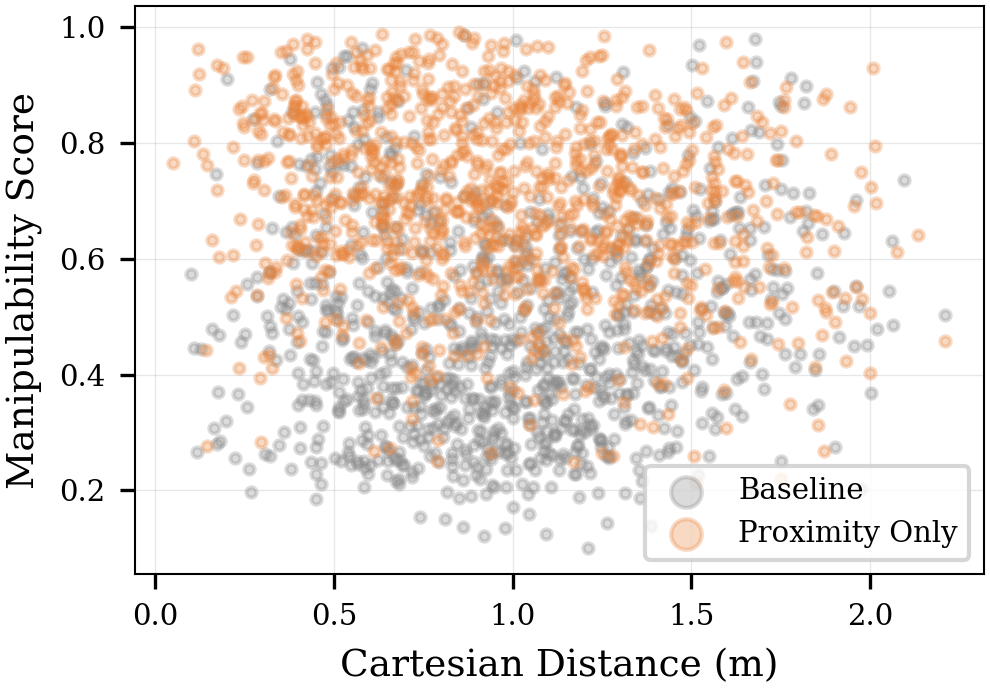
\includegraphics[width=\columnwidth]{fig_manip_vs_dist.png}
\caption{Manipulability score vs.\ Cartesian goal distance for the baseline (grey) and proximity-only (orange) configurations. Each point represents one successful plan.}
\label{fig:manip-vs-dist}
\end{figure}

Figure~\ref{fig:cost-boxplots} shows the per-goal distributions across all eight configurations. The plan time panel~(a) reveals that the baseline has a significantly heavier tail compared to the cost-informed configurations. The manipulability panel~(d) shows a clear separation: configurations that include the proximity term (Prox, \texttildelow Area, \texttildelow Joint, Equal) consistently achieve higher manipulability scores than those without it.

\begin{figure*}[!t]
\centering
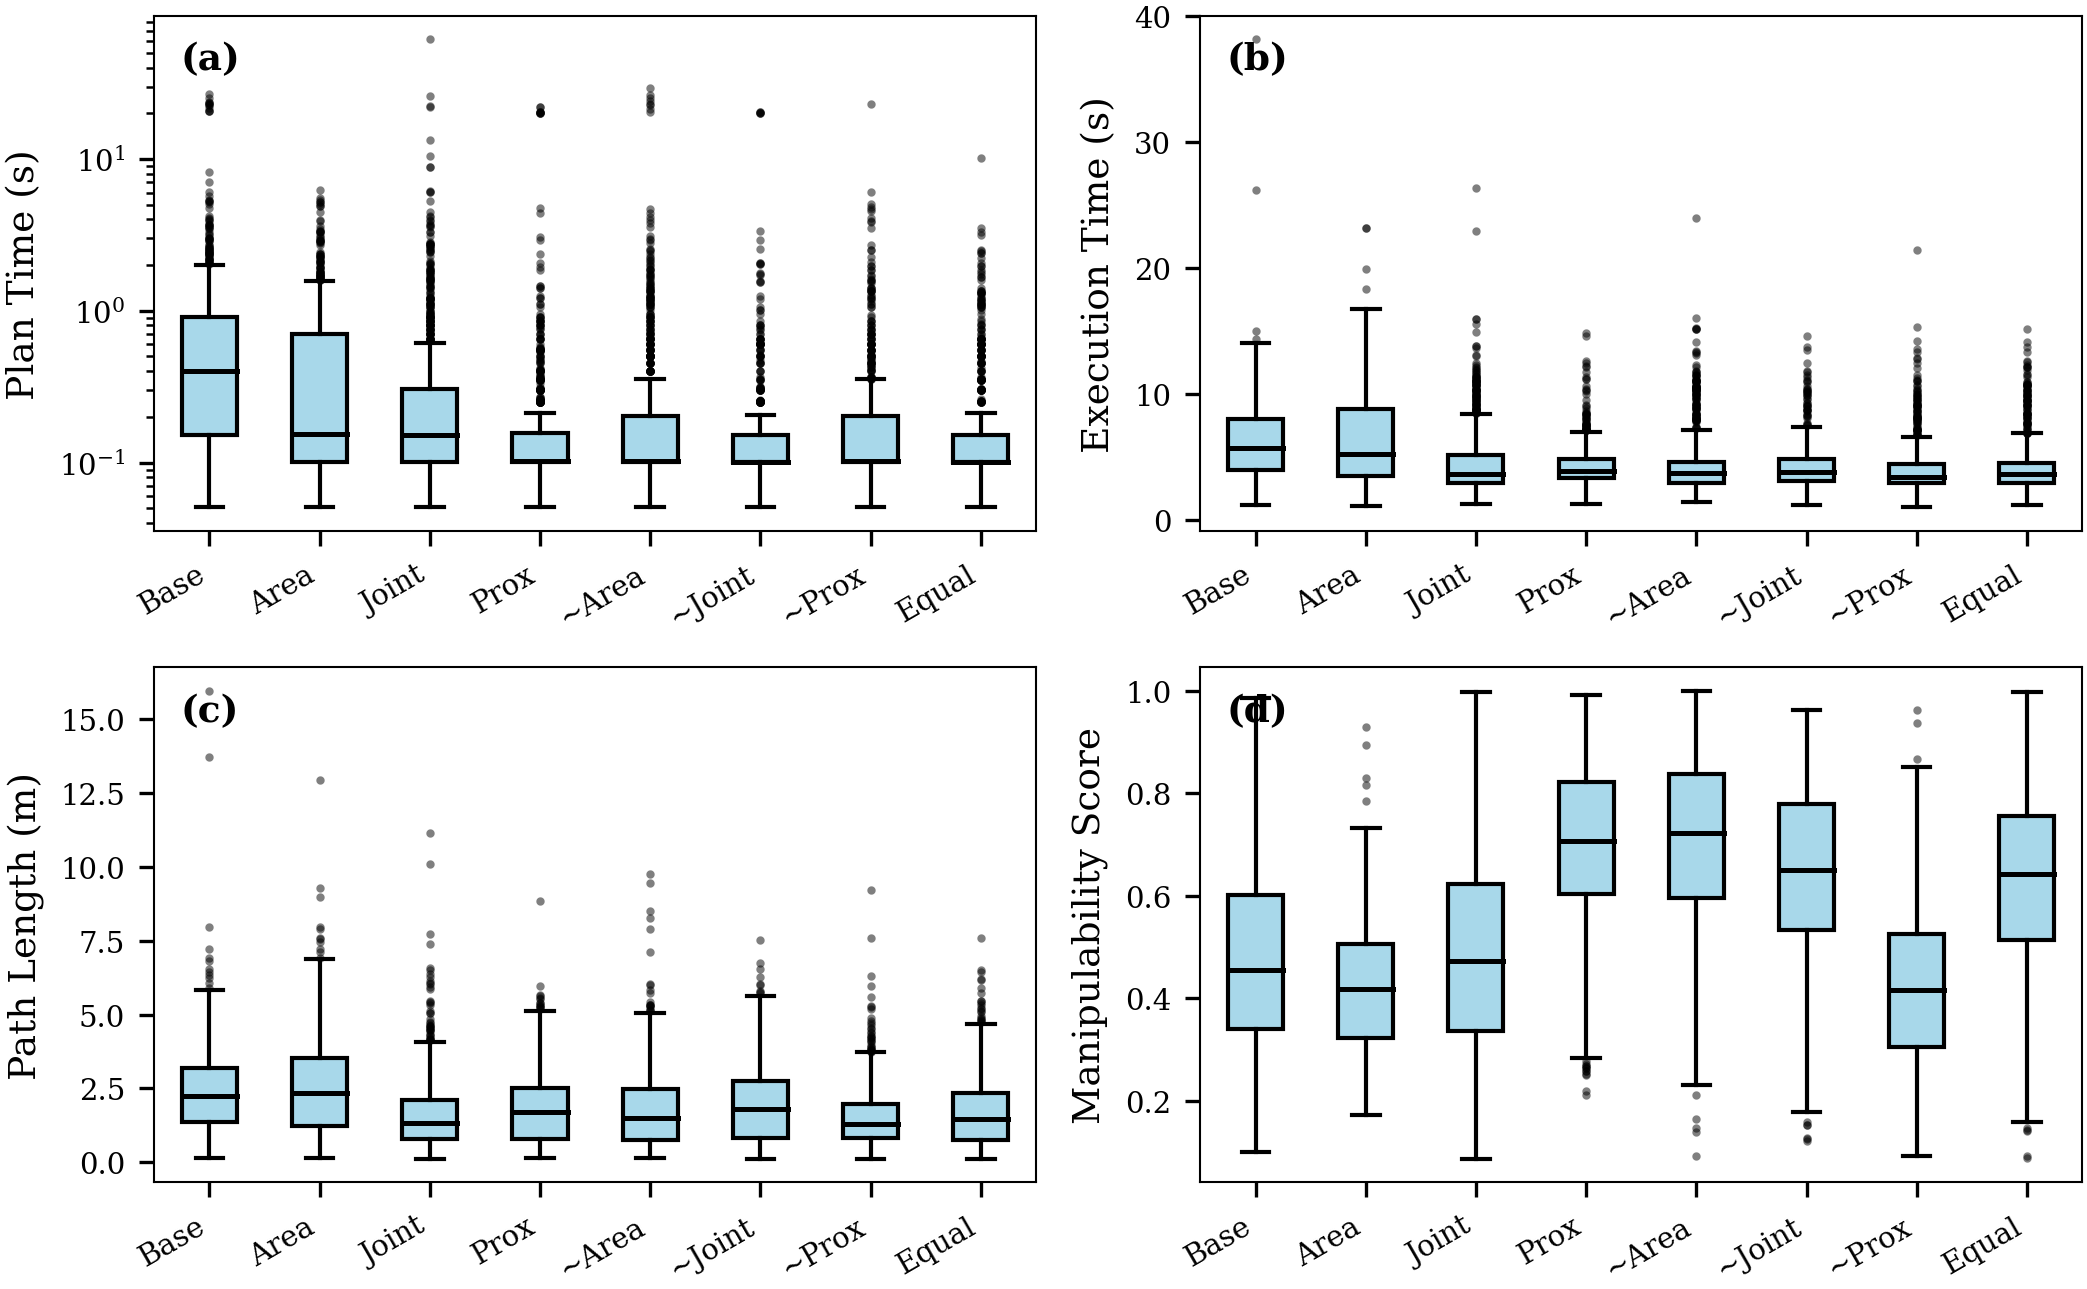
\includegraphics[width=\textwidth]{fig_cost_boxplots.png}
\caption{Per-goal distributions across eight cost function configurations. (a)~Plan time (log scale), (b)~execution time, (c)~path length, (d)~manipulability score. All metrics computed over successful plans only.}
\label{fig:cost-boxplots}
\end{figure*}

Figure~\ref{fig:goal-difficulty} maps the spatial distribution of planning failures across all eight configurations. Goals that failed under multiple configurations cluster near the positive-$x$ workspace boundary, corresponding to extended-reach poses where the arm approaches kinematic limits.

\begin{figure}[!t]
\centering
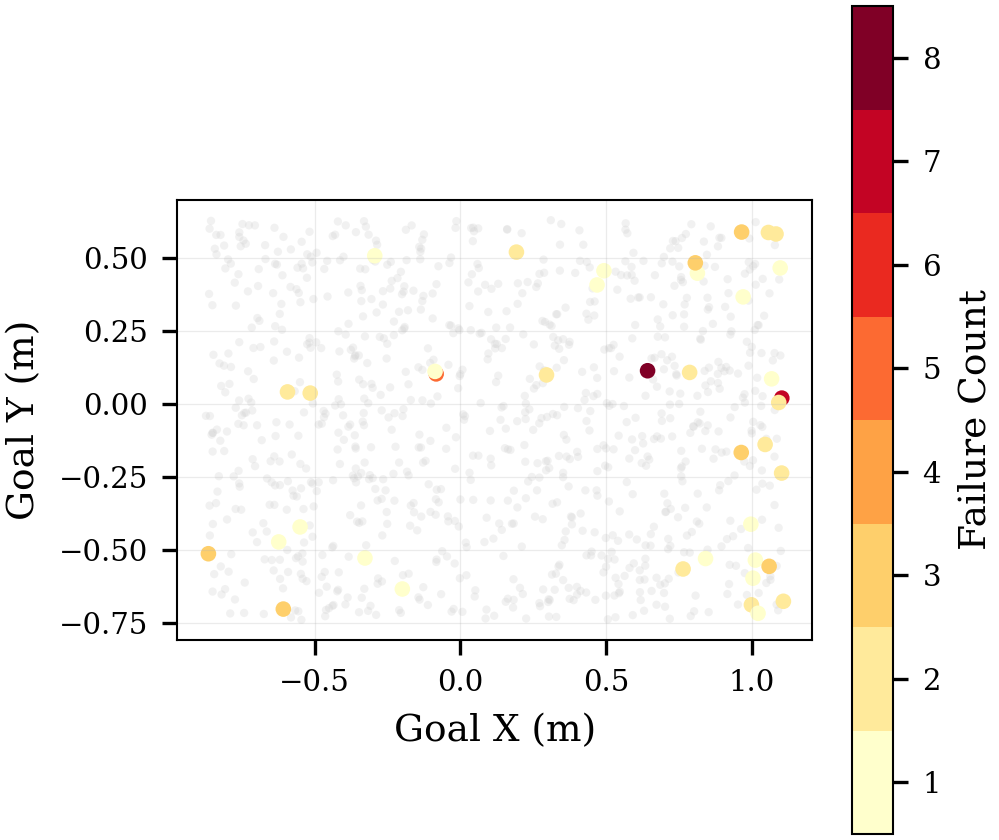
\includegraphics[width=\columnwidth]{fig_goal_difficulty.png}
\caption{Goal difficulty heatmap. Each of 1{,}000 goals is colored by the number of cost configurations (out of 8) that failed to find a plan.}
\label{fig:goal-difficulty}
\end{figure}

\subsection{Vision}
\subsection{Agentic AI}



\section{DISCUSSION}
As in \cite{qu2024robotic}, we observe robots to work significantly slower than human workers. Similar to \cite{qu2024robotic}, we operate the robots far below their maximum speed, but we note that a robot does not necessarily need to be faster than a human to save labor. In this case study, we can reduce the time required to remove all the top-cover screws from 501 seconds with one worker to 400 seconds when the worker is supported by a robot. 

\subsection{Planning}
\subsection{Vision}
\subsection{Agentic AI}

\section{CONCLUSIONS}

We have demonstrated how the agentic AI can both control the robot directly (identifying and disassembling nuts) as well as soliciting human workers for removing screws and the top cover. In the future, we will extend this system to perform a complete disassembly sequence, which will also require humans to change nut-runner bits on the agent's request. In addition to performing a timing analysis and comparing this with manual assembly, we are interested in the human-robot interaction aspects. Here, the proposed solution offers both potential for labor savings as well as consistent instructions, which we wish to quantify by a survey.

Finally, we are interested in extending the proposed solution by an additional mobile manipulator that can perform tasks such as removing screws, changing tools, and transporting small items. 

\addtolength{\textheight}{-12cm}   % This command serves to balance the column lengths
                                  % on the last page of the document manually. It shortens
                                  % the textheight of the last page by a suitable amount.
                                  % This command does not take effect until the next page
                                  % so it should come on the page before the last. Make
                                  % sure that you do not shorten the textheight too much.

%%%%%%%%%%%%%%%%%%%%%%%%%%%%%%%%%%%%%%%%%%%%%%%%%%%%%%%%%%%%%%%%%%%%%%%%%%%%%%%%



%%%%%%%%%%%%%%%%%%%%%%%%%%%%%%%%%%%%%%%%%%%%%%%%%%%%%%%%%%%%%%%%%%%%%%%%%%%%%%%%

\bibliographystyle{ieeetr}
\bibliography{battery}

%%%%%%%%%%%%%%%%%%%%%%%%%%%%%%%%%%%%%%%%%%%%%%%%%%%%%%%%%%%%%%%%%%%%%%%%%%%%%%%%
\section*{APPENDIX}

Appendixes should appear before the acknowledgment.

\section*{ACKNOWLEDGMENT}
Sponsor information withheld for the purpose of double-blind review. 
%This work has been supported by the Advanced Research Projects Agency-Energy (ARPA-E) CIRCULAR Program under cooperative agreement number DE-AR0001966.



%%%%%%%%%%%%%%%%%%%%%%%%%%%%%%%%%%%%%%%%%%%%%%%%%%%%%%%%%%%%%%%%%%%%%%%%%%%%%%%%






\end{document}
